\documentclass[sigconf,review]{acmart}
\acmConference[ICSE 2018]{40th International Conference on Software Engineering}{May 27--June 3, 2018}{Gothenburg, Sweden}
\acmYear{2018}

\usepackage{booktabs} % For formal tables
\usepackage{centernot}
\usepackage{algorithm}
\usepackage{algorithmic}
\usepackage{amsmath,amssymb,amsfonts}
\usepackage{balance}

\usepackage[xcolor=orange]{changes}
\definechangesauthor[name={Claudio Menghi},color=orange]{CM}
\definechangesauthor[name={Sergio Garcia},color=red]{SG}
%\definechangesauthor[name={Patrizio},color=blue]{PP}
\usepackage[colorinlistoftodos,prependcaption,textsize=tiny]{todonotes}
%\newcommand{\sergio}[1]{\todo[color=blue]{\textsf{SG} #1}}

\usepackage[inline]{enumitem}

\newboolean{showcomments}
\setboolean{showcomments}{true} % toggle to show or hide comments
\ifthenelse{\boolean{showcomments}}
{\newcommand{\nb}[2]{
  \fcolorbox{black}{yellow}{\bfseries\sffamily\scriptsize#1}
  {\sf\small$\blacktriangleright$\textit{#2}$\blacktriangleleft$}
 }
 \newcommand{\version}{\emph{\scriptsize$-$working$-$}}
}
{\newcommand{\nb}[2]{}
 \newcommand{\version}{}
}
\newcommand\patrizio[1]{\nb{Patrizio}{#1}}
\newcommand\claudio[1]{\nb{Claudio}{#1}}
\newcommand\sergio[1]{\nb{Sergio}{#1}}
\newcommand\jana[1]{\nb{Jana}{#1}}

\newcommand{\Sync}{\ensuremath{Meet}}
\newcommand{\cla}[1]{\textcolor{red}{{#1}}}

\newcommand{\powerset}{\raisebox{.15\baselineskip}{\Large\ensuremath{\wp}}}
\newcommand{\robot}{\ensuremath{\T}}

\newcommand{\INPUT}{\textbf{Input} }
\newcommand{\OUTPUT}{\textbf{Output} }

\newcommand{\ra}{$\rightarrow$}
\newcommand{\ugh}[1]{\textcolor{red}{\uwave{#1}}} % please rephrase
\newcommand{\ins}[1]{\textcolor{blue}{\uline{#1}}} % please insert
\newcommand{\del}[1]{\textcolor{red}{\sout{#1}}} % please delete
\newcommand{\chg}[2]{\textcolor{red}{\sout{#1}}{\ra}\textcolor{blue}{\uline{#2}}}

\newcommand{\TSi}{{\T_i=(S_i,\init_{i},{A_i} ,T_i)}}
\newcommand{\N}{\mathcal{H}}
\newcommand{\M}{{M}}
\newcommand{\model}{\mathcal{M}}
\newcommand{\I}{\mathcal{I}}
\newcommand{\D}{{D}}
\renewcommand{\O}{\mathcal{O}}

\newcommand{\APs}{\mathbf{\Pi}}
\newcommand{\Lang}{\mathcal{L}} %language
\newcommand{\Set}{\mathsf{S}} %set
\newcommand{\Spec}{\mathbf{\Phi}}
\newcommand{\Epsilon}{\mathcal{E}}
\renewcommand{\i}{\iota}
\newcommand{\Nat}{\mathbb{N}} %natural numbers
\newcommand{\Real}{\mathbb{R}}
\newcommand{\Next}{\mathsf{X}}
\newcommand{\Until}{\mathsf{U}}
\newcommand{\Always}{\mathsf{G}}
\newcommand{\Event}{\mathsf{F}}
\newcommand{\false}{\mathit{false}}
\newcommand{\true}{\mathit{true}}
\newcommand{\trueval}{\ensuremath{\top}}
\newcommand{\falseval}{\ensuremath{\bot}}
\newcommand{\maybe}{\ensuremath{?}}
\renewcommand{\epsilon}{\varepsilon}
\newcommand{\prop}{\pi}
\newcommand{\ie}{{i.e., }}
\newcommand{\eg}{{e.g., }}
\newcommand{\progressive}{\varpi}
\newcommand{\move}{\mathit{move}}
\newcommand{\h}{h}
\renewcommand{\H}{H}
\newcommand{\parti}{\mathit{P}}
\newcommand{\Alpha}{\mathbf{\Sigma}}
\renewcommand{\mod}{\mathrm{\, mod \, }}
\newcommand{\suc}{\mathit{succ}}
\newcommand{\dist}{\mathrm{dist}}
\newcommand{\proj}{\mathrm{proj}}
\newcommand{\parspace}{\vskip 0.05in}


\makeatletter
\newcommand*{\da@rightarrow}{\mathchar"0\hexnumber@\symAMSa 4B }
\newcommand*{\da@leftarrow}{\mathchar"0\hexnumber@\symAMSa 4C }
\newcommand*{\xdashrightarrow}[2][]{%
  \mathrel{%
    \mathpalette{\da@xarrow{#1}{#2}{}\da@rightarrow{\,}{}}{}%
  }%
}
\newcommand{\xdashleftarrow}[2][]{%
  \mathrel{%
    \mathpalette{\da@xarrow{#1}{#2}\da@leftarrow{}{}{\,}}{}%
  }%
}
\newcommand*{\da@xarrow}[7]{%
  % #1: below
  % #2: above
  % #3: arrow left
  % #4: arrow right
  % #5: space left 
  % #6: space right
  % #7: math style 
  \sbox0{$\ifx#7\scriptstyle\scriptscriptstyle\else\scriptstyle\fi#5#1#6\m@th$}%
  \sbox2{$\ifx#7\scriptstyle\scriptscriptstyle\else\scriptstyle\fi#5#2#6\m@th$}%
  \sbox4{$#7\dabar@\m@th$}%
  \dimen@=\wd0 %
  \ifdim\wd2 >\dimen@
    \dimen@=\wd2 %   
  \fi
  \count@=2 %
  \def\da@bars{\dabar@\dabar@}%
  \@whiledim\count@\wd4<\dimen@\do{%
    \advance\count@\@ne
    \expandafter\def\expandafter\da@bars\expandafter{%
    }%
  }%  
  \mathrel{#3}%
  \mathrel{%   
    \mathop{\da@bars}\limits
    \ifx\\#1\\%
    \else
      _{\copy0}%
    \fi
    \ifx\\#2\\%
    \else
      ^{\copy2}%
    \fi
  }%   
  \mathrel{#4}%
}

\everymath{\vadjust{\nobreak\null}}

\makeatletter
\def\old@comma{,}
\catcode`\,=13
\def,{%
  \ifmmode%
    \old@comma\discretionary{}{}{}%
  \else%
    \old@comma%
  \fi%
}
\makeatother

\def\HiLi{\leavevmode\rlap{\hbox to \hsize{\color{yellow!50}\leaders\hrule height .8\baselineskip depth .5ex\hfill}}}

\newif\ifextended
\extendedfalse
%\extendedtrue

\ifextended
\newcommand{\extended}[1]{\textcolor{red}{#1}} 
\newcommand{\notextended}[1]{}
\else
\newcommand{\extended}[1]{}
\newcommand{\notextended}[1]{#1}
\fi

\begin{document}
\title{Towards system development processes for robotic applications }


\author{Sergio Garc\'{i}a}
\email{sergio.garcia@gu.se}
\affiliation{%
  \institution{University of Gothenburg, Gothenburg, Sweden}
  %\city{Gothenburg} 
  %\state{Sweden} 
}

\begin{abstract}
The number of robotic applications that are being developed is increasing exponentially both in industry and academia.
However, those applications do not have common system development process, what leads to the necessity of starting projects from scratch for most of the robot developers.
Thus, developing an application of robotics is always a time consuming task.

In this PhD project, we aim to apply software engineering to robotic systems in order to produce a set of processes, architectural models and methods to be used by developers in order to improve reusability and modularity in robotic applications cutting down the waste of time.
In order to validate our results we make use of a set of service robots that are put to use in different case studies.
\end{abstract}

%
% The code below should be generated by the tool at
% http://dl.acm.org/ccs.cfm
% Please copy and paste the code instead of the example below. 
%
%\begin{CCSXML}
%<ccs2012>
% <concept>
%  <concept_id>10010520.10010553.10010562</concept_id>
%  <concept_desc>Computer systems organization~Embedded systems</concept_desc>
%  <concept_significance>500</concept_significance>
% </concept>
% <concept>
%  <concept_id>10010520.10010575.10010755</concept_id>
%  <concept_desc>Computer systems organization~Redundancy</concept_desc>
%  <concept_significance>300</concept_significance>
% </concept>
% <concept>
%  <concept_id>10010520.10010553.10010554</concept_id>
%  <concept_desc>Computer systems organization~Robotics</concept_desc>
%  <concept_significance>100</concept_significance>
% </concept>
% <concept>
%  <concept_id>10003033.10003083.10003095</concept_id>
%  <concept_desc>Networks~Network reliability</concept_desc>
%  <concept_significance>100</concept_significance>
% </concept>
%</ccs2012>  
%\end{CCSXML}
%
%\ccsdesc[500]{Computer systems organization~Embedded systems}
%\ccsdesc[300]{Computer systems organization~Redundancy}
%\ccsdesc{Computer systems organization~Robotics}
%\ccsdesc[100]{Networks~Network reliability}


%\keywords{ACM proceedings, \LaTeX, text tagging}


\maketitle

\section{Introduction}
\label{sec:introduction}
Service robots are increasingly being involved in human lives. 
They are increasingly used in environments such as houses, airports, hospitals, and offices for performing navigation, transportation, and manipulation tasks. 
The World Robotic Survey~\cite{wrs:online} estimated 35 million indoor service robots to be sold by 2018, accumulating a sales value of \$12 billion since 2015. 
%The global sales of household and personal robots is expected to grow by 23.5\% per year~\cite{sheng:online}. 
This increase is accompanied with huge progress in robot technology. %, especially in image processing, planning, control, and collaboration. 
Software engineering is key to sustaining this new technology.

A robot typically performs specialized tasks; however, some tasks are highly complex and require a team of robots, whose capabilities (e.g., perception, manipulation, and actuation) are coordinated and supervised. 
Such teams also need to adapt to changes, such as of the environment, of the desired tasks, or of the robot (e.g., hardware failures). 
These demands drive the complexity of robot control software relying on appropriate software architectures. 
To tackle this complexity, we need to rethink design processes~\cite{Lee2008} by properly managing system integration and raising the abstraction levels, addressing qualities like evolvability~\cite{Perez2008}, configurability~\cite{Gamez2013563}, scalability and dependability.

%The PhD project presented in this paper 
Our work is involved in the Co4Robots~\footnote{http://www.co4robots.eu/} European project.
Being part of this project allow us not only to formulate but also to validate our research questions in real-world scenarios.
%According to~\cite{roadmap}: ``Usually there are no system development processes (highlighted by a lack of overall architectural models and methods). 
%This results in the need for craftsmanship in building robotic systems instead of following established engineering processes".
According to~\cite{roadmap} there are no system development processes for robotic applications.
%In fact, most of the robotic applications developed nowadays have to be started from scratch without following well-engineered methods.% to help in the process.
In fact, robotic applications nowadays are started from scratch without following well-engineered methods.
In this context the aim of the Co4Robots project is to establish systematic engineering process to facilitate the development of the software for animating robotic systems through the creation of reusable robot building blocks with well-defined interfaces and properties. 

The research conducted during the present project will be split in two parts.
The first one defines the best practices for engineering software robotic applications.
During this period we studied the current software engineering practices for both single and multi-robotic systems.
Furthermore, throughout this part of the research we will develop the platform that will be allocated within every robot of our applications.
An instance of our \emph{Software platform} will be deployed on each robot.
It will integrate the \emph{Software architecture} of the whole system and  the \emph{Configuration facilities}, which provide the required tools for configuring our architecture.% both at design and run-time.

The second part of the research aims to support the \emph{choreography} of robotic applications.
It is considered future work that will be tackled once the platform is completely addressed.
In this context, choreography means the way of representing and controlling the interactions between multiple services of a system in a decentralized way.
%The main expected outcome of this part is to perform 
Our goal is to perform the choreography of a deployed team of potentially heterogeneous robots in dynamic environments with the presence of human beings.
In order to do so, issues as \emph{Emergent properties} ~\cite{DeAngelis2016} and selecting the most suitable \emph{Collaborative adaptation}~\cite{Yan2013} techniques must be addressed.

\textbf{Research Questions.} 
Based on the division of the project, we state the following research questions:
\begin{itemize}
\item[RQ1] Which are the current software engineering practices for engineering robotic applications and which are their limitations?
\item[RQ2] Which software engineering practices can be developed to improve the process of engineering robotic applications?
\item[RQ3] Which are the applicable strategies to manage a heterogeneous robotic application with only partial knowledge of a dynamic environment?
\end{itemize}

\textbf{Contributions.} 
Our contributions are listed in the following:

\begin{enumerate}
\item Definition of a software architecture able to structure a robotic team;
%\item Validation of the architecture in a real-world scenario
\item Implementation of a software platform where all the algorithms and tools developed can be plugged in;
\item Definition of configuration mechanisms to enable \emph{start-up configuration} and \emph{run-time configuration};
\item Integration of an approach based on ROS+REST for the internal communication between robots;
\item Development of the algorithms in charge of managing the robotic team, based on management of emergent properties and selection of collaborative adaptation techniques.
%\end{enumerate}
\end{enumerate}

At this moment the software architecture and the communication mechanisms are already developed.
The software platform is being continuously developed and we intend to start dealing with the configuration facilities in the near future.
The development of the algorithms in charge of managing the robotic team are planned to be addressed during the second part of the project.

\textbf{Organization.} 
Section~\ref{sec:approach} describes our research approach and answers the first RQ. %of the current work and answers the first RQ.
In Section ~\ref{sec:single} we present the process that we follow for engineering robotic applications and answer RQ2.
Then, in Section~\ref{sec:multi} we explain our plan for managing a robotic team while answering RQ3.
In Section~\ref{sec:related}, we introduce different works with a similar scope and position our research.
Section~\ref{sec:validation} explains our validation plan.
Section~\ref{sec:conclusion} concludes with final remarks.

\section{Research approach}
\label{sec:approach}
The plan within this project is to split the work not only regarding topics but time in two parts:
\begin{enumerate*}
\item the first part, focused on the study of current practices for engineering robotic applications (RQ1) and the development of the framework allocated within each robot (RQ2); and
\item the second part, focused on collaboratively managing a team of robots (RQ3).
\end{enumerate*}

This project is being developed closely with the industry because it is embedded in the Co4Robots European project.
The main goal of this project is to deploy a robotic application in a ``domestic" environment such as hospitals, hotels, airports, etc.
These environments will be considered as dynamic and will also count with the presence of human beings.
We consider that robotic applications must be able to accomplish complex missions with a systematic, real-time, decentralized methodology.
Furthermore, a robotic application could be composed by a team of potentially heterogeneous robots.
For this reason, the robots must have integrated a set of perceptual capabilities that enables them to localize themselves and estimate the state of their highly dynamic environment in the presence of strong interactions and in a collaborative manner.
That is, robots must not only interact between them, but also with human beings.

In order to learn which are the current practices for developing robotic applications we performed an extensive research in the field.
We also plan to conduct empirical studies such as interviews with different companies, starting with the industrial partners of Co4Robots.
With this steps we expect to answer RQ1 and also to figure out which are the limitations of such practices.  

A not negligible task within this project is to decouple the research made just for Co4Robots and the one intended for the whole PhD.
While the framework development outcomes is common for both our own research and the Co4Robots' , our outcomes of the collaborative adaptation part are expected to reach far beyond results than the intended by Co4Robots.
%For example, for our own research we plan to manage a team of robots acting under some defined collaborative strategies and adapting to emergent properties.





\section{Engineering robotic applications}
\label{sec:single}
Currently, our main focus lays on the RQ1, learning, defining and differencing between software engineering practices regarding single-robot and multi-robot systems.
In order to answer this question we divided the first part of our research into different tasks.
First, we defined the software architecture that defines our system.
Then, we will implement configuration facilities that enables the customization of the different components that compose the architecture.
Finally, we will develop the software platform where the previous work is implemented.

\subsection{Software architecture}

Our software architecture, Self-adaptive dEcentralised Robotic Architecture (SERA) is already defined.
As its name indicates, it supports a real-time decentralized robot coordination to accomplish missions with teams of robots. 
Furthermore, it is self-adaptive, responding to different changes by computing new strategies to achieve the desired goals.
SERA is inspired by and extends concepts of existing proposals for robot software architectures from the literature. 
Specifically, we inspected architectures identified by a mapping study of Ahmad et al.~\cite{Ahmad201616}, which investigated software architectures for robotics systems to identify and analyze the relevant literature based on 56 peer-reviewed papers.
The aforementioned architecture is three layers architecture that is strongly influenced by the well-known work of Kramer and Magee~\cite{kramer}.
It has the same structure, but we also added a new item that works as a central station.
It is important to remark that the aim of our project is to build a system that can be easily used by not technical users, so we had to define a way for them to command the missions to the robotic team.
The central station is just used during design-time in order to allocate a graphical interface to be used by a final user.

We defined SERA by first conceiving an architecture for a single robot. 
It means that all components, interfaces and units were defined for a single robot architecture. 
Then, we extended and refined it in order to iteratively extend and refine the architecture towards enabling communication among robots and collective adaptations. 
Thus, all the robots have a instantiation of the reference architecture but are also able to communicate and share information with the rest of the team, making possible the collective adaptation. 

SERA was already tested during an Integration Meeting of the project, where it demonstrate that can support the performance of a robot achieving different complex missions ---i.e. collaborative transportation with an human being, autonomous driving in a dynamic environment.

%\begin{figure*}[!t]
%\begin{center}
%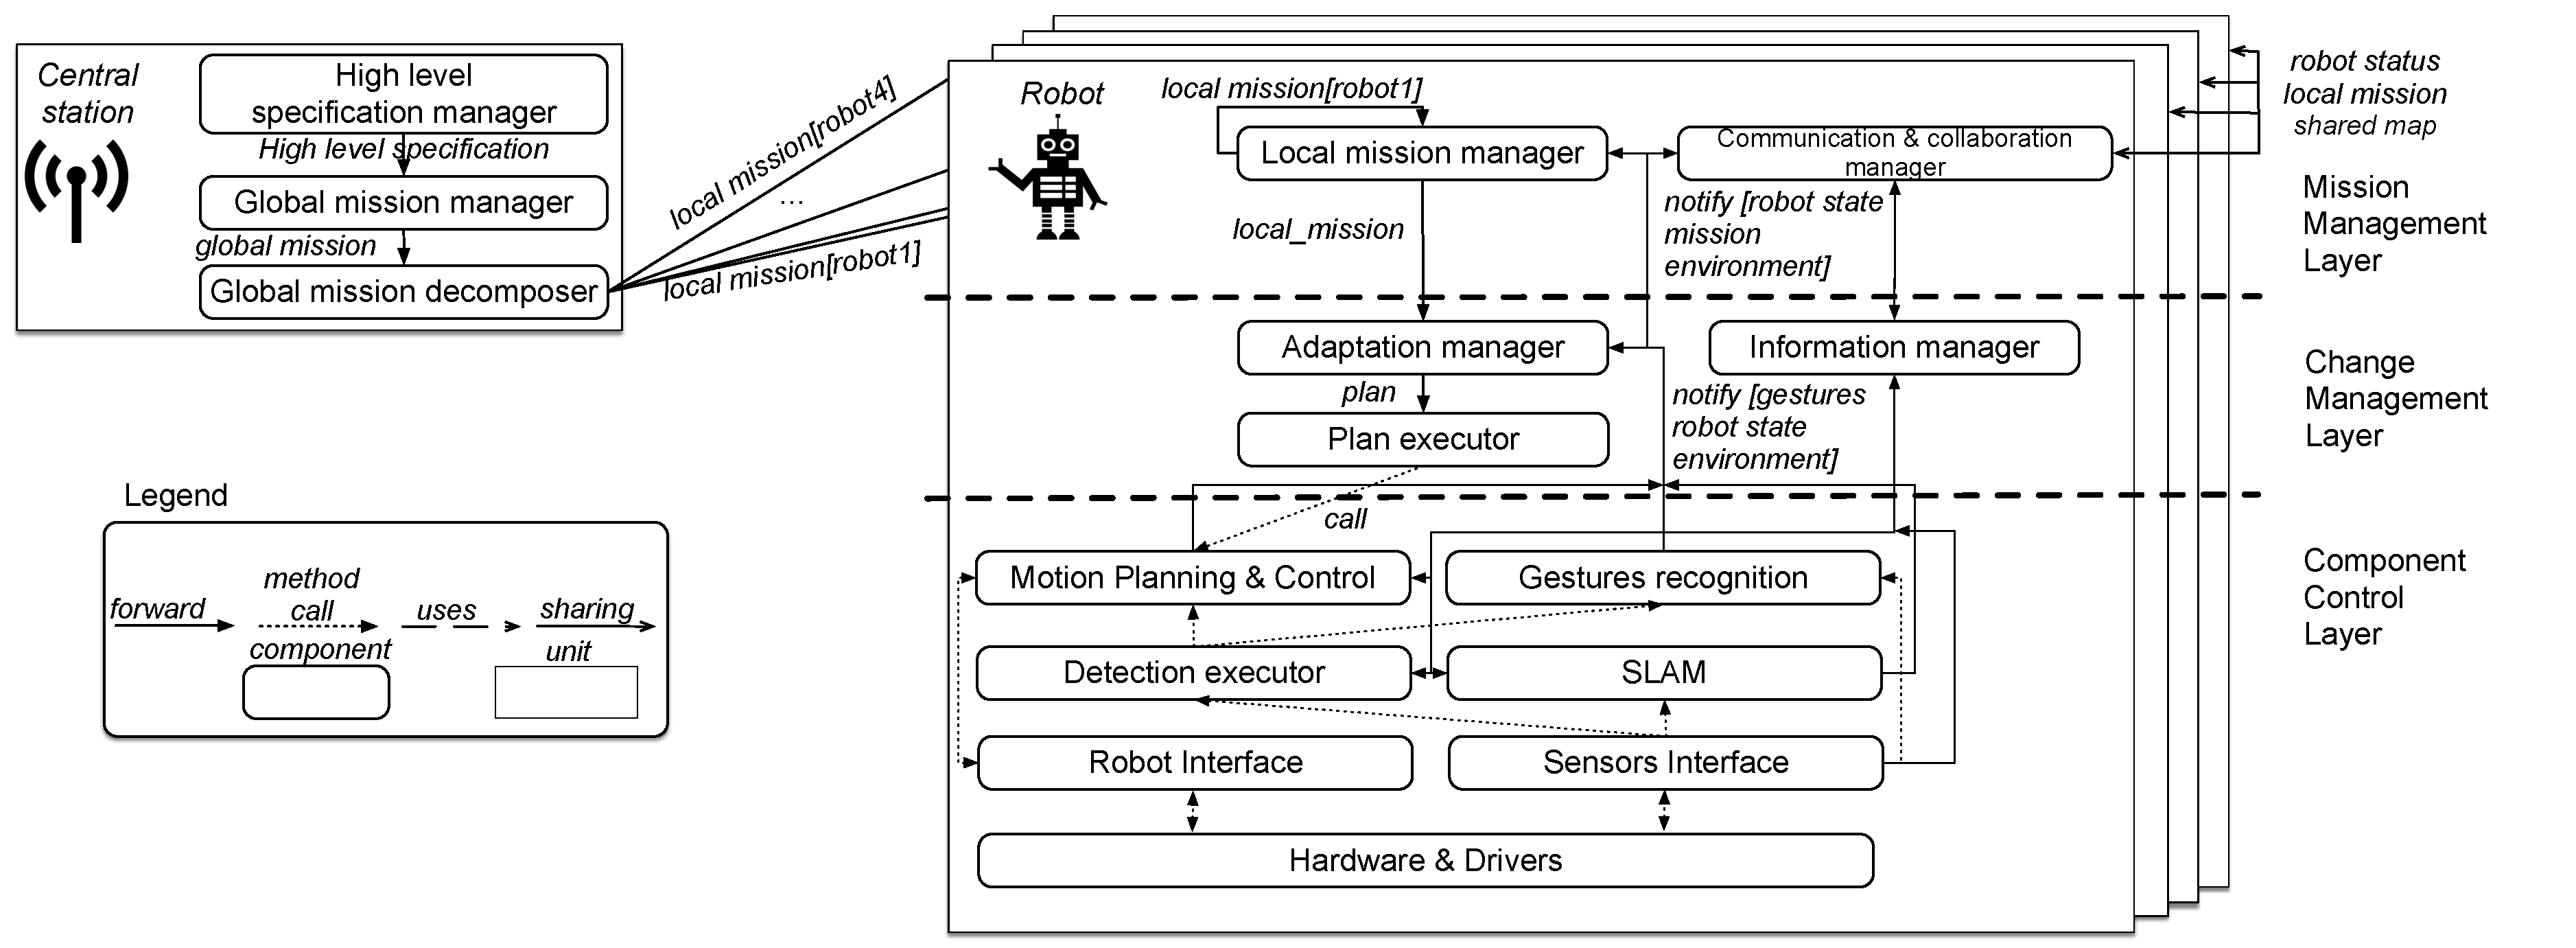
\includegraphics[width=1\linewidth]{Figures/InstanceMultiRobot_Graffle.pdf}
%\caption{Software architecture.}
%\label{fig:arch}
%\end{center}
%\end{figure*}

\subsection{Configuration facilities}

Since the components of our architecture are exchangeable our next short-term goal is to define configuration facilities that can be applied to our system depicted in the architecture.
It will allow to our applications to support two things:
\begin{enumerate}
\item Being customizable at design-time, so we can configure its components based on the requirements of our context (i.e. hardware installed in each robot, environment where they will be deployed, etc.)
\item To self-adapt or self-configure at run time, so each robot can apply changes in its configuration based on emergent events of the environment or failures of their system.
\end{enumerate}

In order to do so we will implement pluginlib~\footnote{http://wiki.ros.org/pluginlib}, a package that uses the ROS build infrastructure and provides tools for writing and dynamically loading plugins.

\subsection{Software platform}

As explained before, the Software platform will integrate the Software architecture and all the tools and software created by developers and also the configuration facilities.
Regarding the architecture, SERA follows the component-based style, so the main robotic functionalities are encapsulated in different modules or "components".
The platform is also a collection of such components, a kind of library.
All this components are developed abstracting the communication capabilities since we rely on the interfaces defined in the architecture.
It not only significantly reduces the complexity of the code but also triggers the modularity of our system making possible exchanging the components that conform our architecture.

We not only plan to control the performance of the system that is running in each robot but also its behaviour.
Thus, the usage of high-level behavior engine, flexibly applicable to numerous systems and scenarios is mandatory.
FlexBe~\cite{Schillinger2016} not only provides a way of defining the behaviour of the robot in different scenarios (as of the study cases) by means of a work flow, but also a graphical interface that simplifies enormously this task.
FlexBe encapsulates functionalities of the robotic application, as our architecture does within components, and provides a way of orchestrate them so we keep the modularization of our system.
As with ROS, an instantiation of FlexBe will be deployed in every robot.
The integration of FlexBe is driven for the necessity of a software development methodology as MDE in our project.
It improves the modularity, variability and reusability of our system facilitating the development of the software for animating robotic systems through the creation of reusable robot building blocks with well-defined interfaces and properties.

Finally, in order to communicate each robot with its teammates we implemented an approach based on ROS+REST.
So, using a suitable component that works as an interface we are able to send messages in form of services between robots.
In this way, each robot has an instance of ROS running in their own local environment so we can deploy a whole team of robots avoiding a central master node and the problems related with this approach (i.e. bottleneck issues, less robustness facing failures of a node, etc.), specially working with the ROS middleware.



\section{Supporting the choreography of robotic applications}
\label{sec:multi}
As stated before, we plan to split the work related with this PhD project in two parts: 
\begin{enumerate*}
\item the first part, focused on the framework allocated within each robot; and
\item the second part, focused on the choreography of a team of robots.
\end{enumerate*}

Therefore, our future work will be focused on trying to find an answer to the RQ2.
In order to achieve it, a detailed study of the current state of the art of features involved with multi-robot choreography such as emergent properties or collaborative strategies must be performed.
Nevertheless, since our plan is to continously integrate all the obtained knowledge into the research the framework developed during the first division of the project will be used and tested through this part as well.
Furthermore, due to the tools created for the robot orchestration will be tested on real robots we still will need to deploy the software platform and its functionalities on each of them.
An architectural overview of the whole research is depicted in Figure~\ref{fig:overview}.
\sergio{fix figure adding dotted lines! rename to collective adaptation!}
In this figure the expected final system is represented in a schematic way.
It represents blocks that emulates the contents of each robot that are unfolded, representing a team of robots.
The communication methodology is also represented in the figure, explaining how the robots will communicate.
Then, the properties that we plan to study in order to perform the orchestration are also depicted on top of the previous explained blocks. 
In the following we explain those properties.

\begin{figure}[!t]
\begin{center}
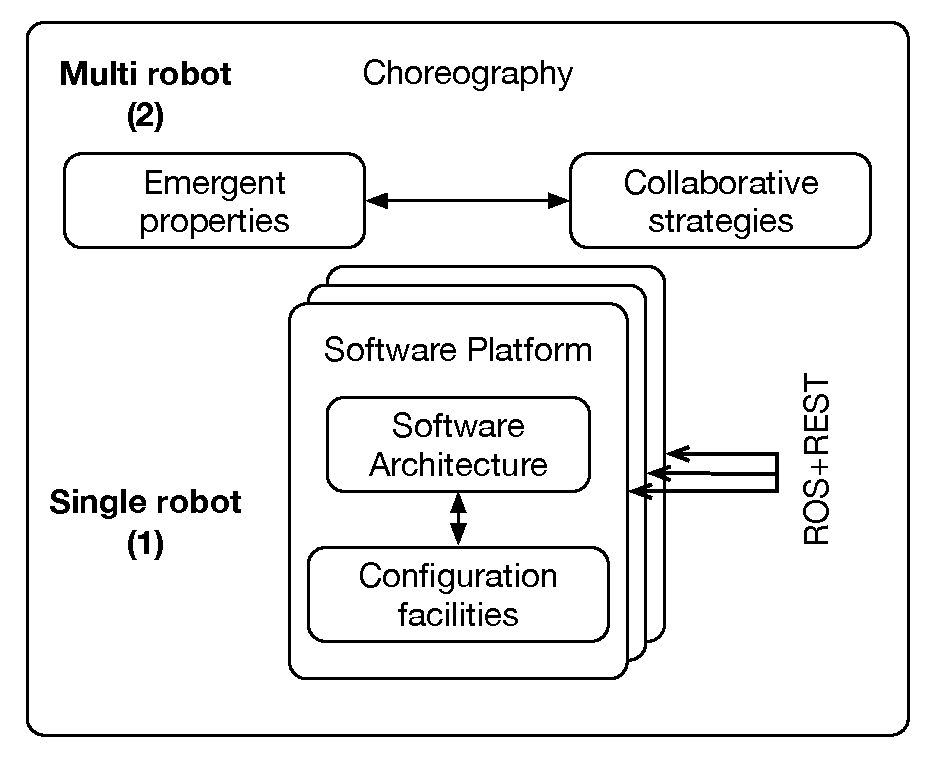
\includegraphics[width=1\linewidth]{Figures/researchv2.pdf}
\caption{Architectural overview of the final system.}
\label{fig:overview}
\end{center}
\end{figure}

\section{Related work}
\label{sec:related}
In this section we discuss related work with respect with our two proposed Research Questions.

Our robotic application will be based on ROS~\cite{Quigley2009} and some functionalities will be build on top of it. 
ROS is an open-source meta-operating system for robots. 
It provides a communication layer above the Linux host operating system that supports the execution of components in a distributed system. 
ROS offers message-based peer-to-peer communication infrastructure supporting the integration of independently developed software components, called ROS nodes, that are organized into a graph.

The benefits for using ROS are many and one of them is the flexibility that this tool provides to the developers.
However, this flexibility could result in a development process based on ad-hoc solutions rather than being based on a systematic engineered approach. 
Obviously, it decreases the modularity and reusability of the developed system and makes its development process to take longer due to many of its applications will have to be generated from scratch. 
Furthermore, ROS has some limitations, some of them recognized by their developers~\footnote{http://design.ros2.org/articles/why\_ros2.html}.
ROS2 is supposed to solve these previous problems and to substitute ROS1 in a near future, but since it was just released and there are not yet all the contents that were available for ROS1 we opted for keep using ROS1.

Architectures
	Decentralized
	Multi-agent
	Not SOA, microservices, cloud container

Collaborative adaptation


\section{Validation}
\label{sec:validation}
In order to validate the code and artifacts developed for Co4Robots, the committee defined a set of study cases for the project proposal.
Our framework builds upon various cases of base interactions between agent pairs of different types. 
The considered inter-agent interactions are:
\begin{itemize}
\item[Case A] physical guidance by a human for the transportation of an object carried by a robot;
\item[Case B] collaborative grasping and manipulation of an object by two agents;
\item[Case C]collaborating mobile platform and stationary manipulator to facilitate loading and unloading tasks onto the mobile platform; and
\item[Case D] information exchange between a human giving orders and a robotic agent. 
\end{itemize}

Therefore, one the most important ways of testing and validating of most of the results obtained in this research are the previously stated study cases.
For each study case, the Co4Robots consortium holds a \emph{Milestone meeting} in order to test all the developed tools.
It allow us not only to test our research outcomes in real robots working in real-world scenarios but also to discuss with the rest of the developing stakeholders involved in the project and collecting valuable feedback.
The outline of the approach that we are currently follow for our approach and the validation is as follows:
\begin{enumerate}
\item Personal work alternated with internal meetings.
\item Previous validation by means of simulating scenarios.
\item Presentation of achieved work to the Co4Robots committee and collection of feedback.
\item Correction of work based on feedback.
\item Validation during Milestones and Integration Meetings.
\item Documentation for deliverables requested for every task within each Workpackage of the project.
\end{enumerate}







\section{Conclusions}
\label{sec:conclusion}
Software engineering can be the key technology needed for the improvement of applications developed for robotic systems.
Robots are nowadays a trend, but without well-defined engineering process for the researchers to follow most of the projects are started from scratch and not time neither cost efficient.
In this project we aim to tackle those problems while validating the premises and results with real-world scenarios where real robots work in a collaborative way.

Furthermore, we plan to perform a detailed research in the state of the art

\section*{Acknowledgments}
\label{sec:Acknowledgments}

EU H2020 Research and Innovation Programme, grant 731869 (Co4Robots).


\balance

\bibliographystyle{ACM-Reference-Format}
\bibliography{sigproc} 

\end{document}
